\documentclass[UTF8,11pt,a4paper]{ctexart}
\usepackage[margin=1in]{geometry}
\usepackage{graphicx}
\usepackage{booktabs}
\usepackage{amsmath}
\usepackage{hyperref}
\usepackage{float}

\title{\textbf{高 Beta 全日照边界工况下的小卫星被动热控设计与散热器尺寸权衡研究}}
\author{\textbf{热控系统主任设计师} \\ \textit{空间系统工程部}}
\date{}

\begin{document}

\maketitle

\begin{abstract}
本报告针对运行于 600 km 圆轨道晨昏太阳同步轨道（SSO）的高功耗 6U 技术验证立方星，开展了初步被动热控设计与散热器尺寸权衡分析。晨昏 SSO 轨道的特殊几何特性导致卫星在至日期间处于高 Beta 角（$\beta = 74^\circ$）状态，整星处于不进入地球本影的“全日照”极端外部热环境中，对航电和电池组带来极高的超温风险。本报告提出了 \textbf{被动热控重设计 v2 方案}，无需依赖复杂的活动关节散热器或热管等主动/两相装置，仅通过合理的物性表面分区（AZ-93 硅酸盐白漆与银 FEP 二次表面镜胶带散热器）、朝向物理学原理（将散热面置于永久背阴的 $-Y$ 侧面）以及光电转换能量扣除模型进行整星热平衡重设计。散热器面积扫频分析表明，采用 $0.02\text{ m}^2$ 散热面积可在保证极端热工况安全裕度（航电峰值 $39.2^\circ$C）的同时，最大程度限制冷工况下生存加热器的能耗（$5.92$ Wh/轨道），是系统级的最优被动热设计。
\end{abstract}

\section{引言}
现代小卫星的集成度不断提高，内部电子单机和载荷的功耗大幅上升。对于标准的 6U 立方星（尺寸 $10\text{ cm} \times 20\text{ cm} \times 30\text{ cm}$），在特殊的轨道环境下极易发生过热失效。

本项目的基准轨道为 600 km 晨昏太阳同步轨道，轨道倾角 $\approx 97.8^\circ$。在至日期间，由于轨道面与太阳矢量的夹角很大，太阳 Beta 角可高达 $74^\circ$，超出了本轨道的遮阴临界角（$\approx 66.07^\circ$），导致卫星处于 100\% 全日照状态。轨道的几何特征与日照条件如图 1 所示。

\begin{figure}[H]
\centering
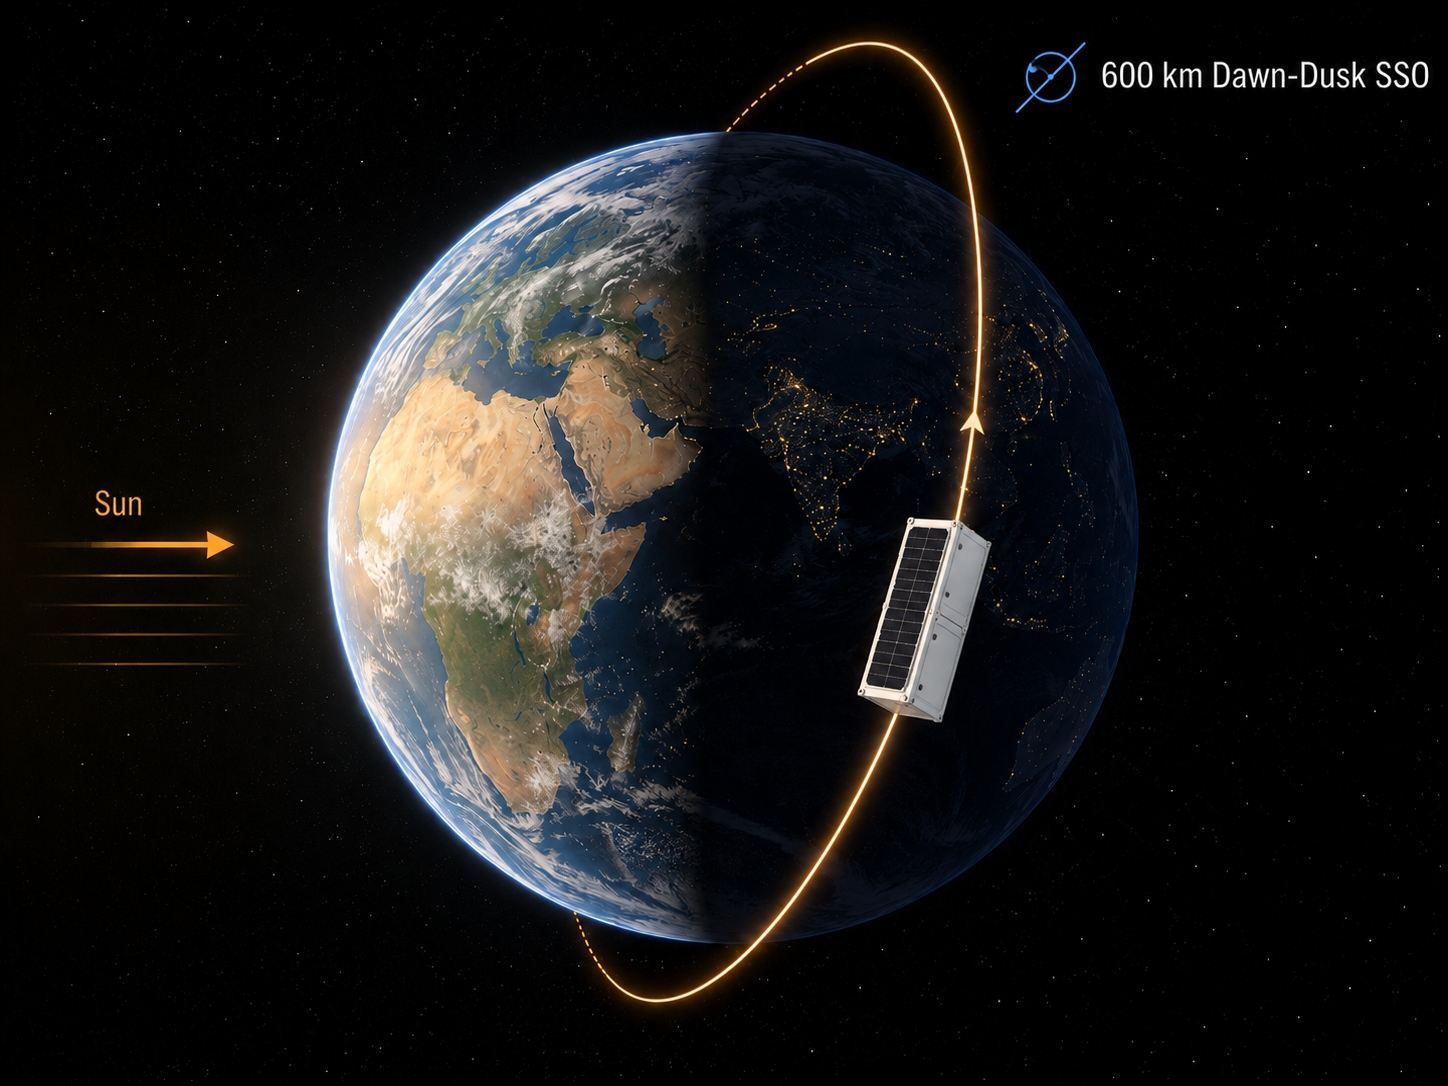
\includegraphics[width=0.75\textwidth]{sso_orbit.png}
\caption{600 km 圆轨道晨昏太阳同步轨道（SSO）几何示意图，展示了侧向面板接收的持续太阳辐射矢量。}
\end{figure}

\section{热控要求与单机物性参数}
卫星各结点的热容和工作限制温度严格遵照航天规范和单机性能，详细参数见表 1。

\begin{table}[H]
\centering
\caption{各热结点质量、热容及工作限值}
\vspace{0.2cm}
\resizebox{\textwidth}{!}{%
\begin{tabular}{lccccc}
\toprule
\textbf{结点 ID} & \textbf{质量 [kg]} & \textbf{比热 [J/kg$\cdot$K]} & \textbf{工作下限 [$^\circ$C]} & \textbf{工作上限 [$^\circ$C]} & \textbf{内部功耗 [W]} \\
\midrule
电池包 (Battery) & 1.5 & 800.0 & -10.0 & 45.0 & 0.5 \\
航电单机 (Avionics) & 1.0 & 900.0 & -20.0 & 60.0 & 10.0 -- 15.0 \\
载荷相机 (Payload) & 2.0 & 900.0 & -10.0 & 50.0 & 0.0 -- 15.0 \\
结构框架 (Structure) & 3.0 & 900.0 & -40.0 & 80.0 & 0.0 \\
散热板 (Radiator) & 0.5 & 900.0 & -100.0 & 100.0 & 0.0 \\
外壳板 (External Shell) & 1.5 & 900.0 & -100.0 & 100.0 & 0.0 \\
\bottomrule
\end{tabular}%
}
\end{table}

卫星 6 结点集集集总参数热网络架构、导热耦合路径 $G_{ij}$ 以及外部热载荷接口关系如图 2 所示。

\begin{figure}[H]
\centering
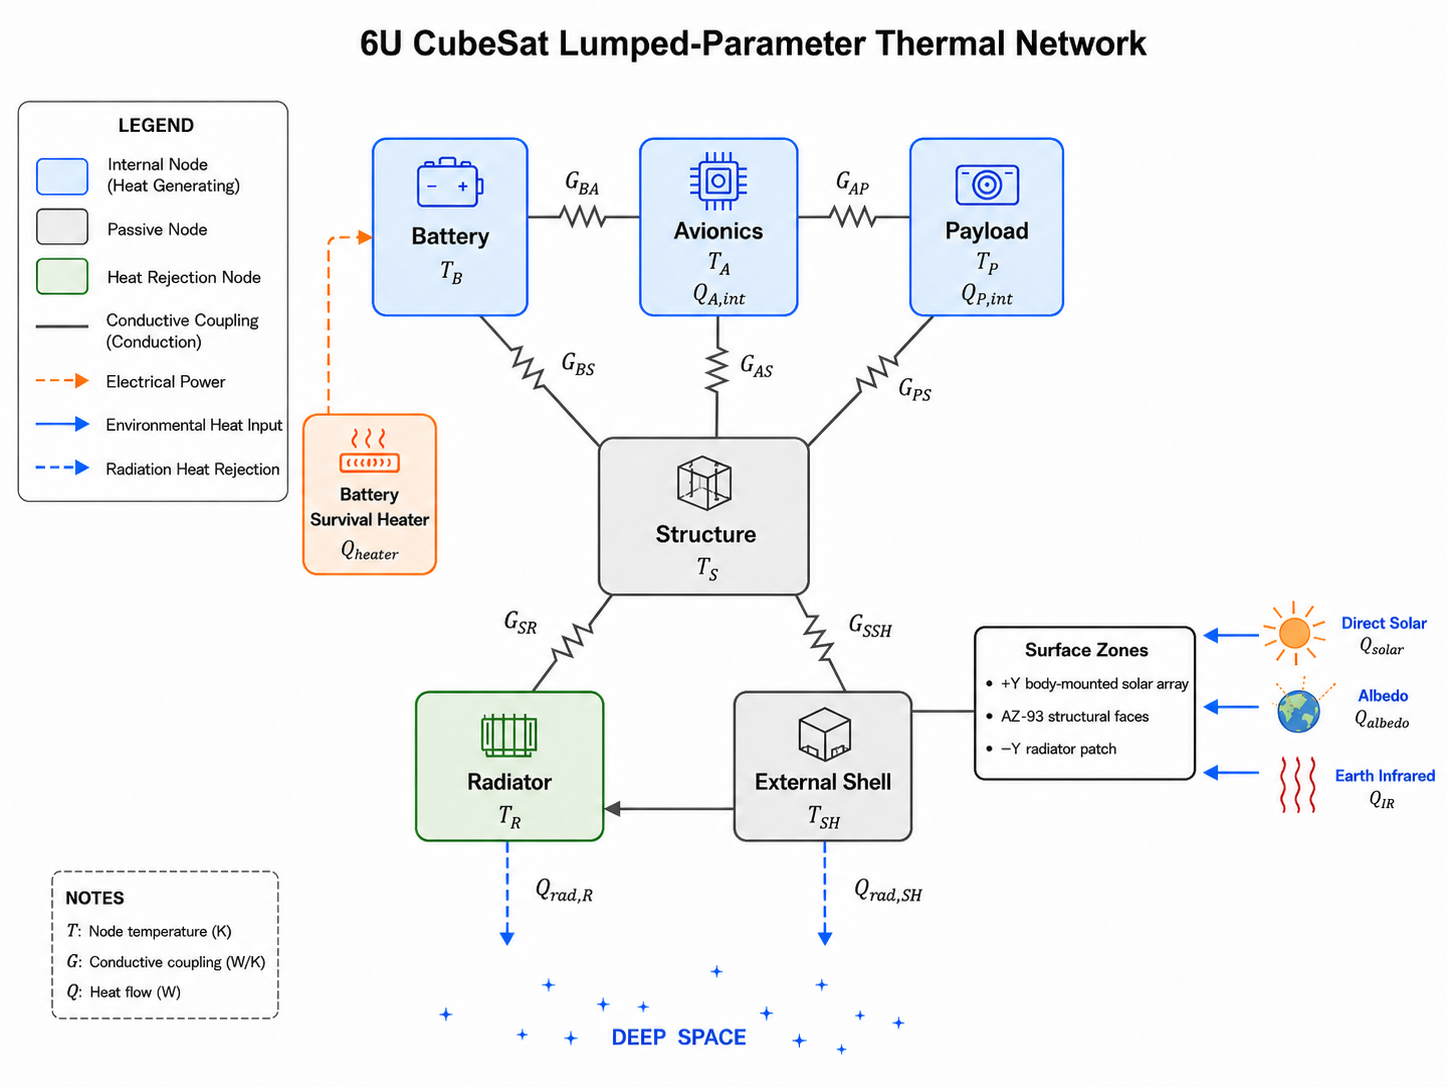
\includegraphics[width=0.75\textwidth]{thermal_network.png}
\caption{6 结点集总参数热网络拓扑图，展示了结点间的导热通路及外部辐射载荷耦合关系。}
\end{figure}

\section{材料库与光学特性}
本项目热分析中使用的所有涂层及物性数据均直接引自 \href{https://www.nasa.gov/smallsat-institute/sst-soa/thermal-control/}{NASA SmallSat State of the Art (SoA) Thermal Control} 官方网页，特别是其中的 Table 7-3 和 Table 7-4。具体的材料目录如表 2 所示。

\begin{table}[H]
\centering
\caption{材料物理参数与太阳吸收率/红外发射率（引自 NASA 官方数据）}
\vspace{0.2cm}
\resizebox{\textwidth}{!}{%
\begin{tabular}{llcccl}
\toprule
\textbf{材料名称 (Material ID)} & \textbf{设计用途} & \textbf{$\alpha_s$ (BOL)} & \textbf{$\epsilon_{IR}$} & \textbf{NASA 数据源} & \textbf{工程说明} \\
\midrule
AZ-93 Silicate & 外壳被动保护 & 0.16 & 0.90 & Table 7-3 & 无机白漆，低吸收、高发射 \\
0.005$''$ FEP/Ag/Inconel & 散热板表面 & 0.07 & 0.79 & Table 7-4 & 二次表面银 FEP 胶带，极低吸收 \\
VDA/200HN/PSA & 隔热对比材料 & 0.08 & 0.03 & Table 7-4 & 镀铝聚酰亚胺胶带，低发射率 \\
Z306 Polyurethane & 吸热对比漆 & 0.92 & 0.89 & Table 7-3 & 哑光黑漆，高太阳吸收率 \\
solar\_cell\_assembly & 太阳能电池翼板 & 0.73 & 0.82 & Section 7.1 & 贴装单体太阳电池组件 \\
\bottomrule
\end{tabular}%
}
\end{table}

\section{基准设计失效分析}
在初始的 baseline 方案中，多块外壳面板涂覆了高太阳吸收率的黑漆（$\alpha = 0.92, \epsilon = 0.89$）以作为太阳能电池翼板。在全日照热工况下，由于卫星表面吸热巨大，导致多处单机超温失效（电池达 $80.6^\circ$C，航电达 $81.6^\circ$C）。此外，分析证明如果误用低发射率的多层隔热反射膜（如 VDA 胶带，$\epsilon = 0.03$）作为散热板，会因无法有效辐射散热导致热量在内部积聚，使航电飙升至 $104.1^\circ$C 造成损毁。

\section{被动热控重设计 v2 方案}
为在资源受限的小卫星上实现低成本被动热设计，我们实施了以下重设计方案：
\begin{itemize}
    \item \textbf{物性表面分区 (Thermal Zoning)}：将 5 块非发电表面喷涂 AZ-93 硅酸盐白漆（$\alpha=0.16, \epsilon=0.90$），在降低太阳吸热的同时向太空提供高效放热路径。
    \item \textbf{散热板背阴朝向物理学 (Radiator Orientation)}：在 600 km 晨昏轨道中，$+Y$ 侧面永远面向太阳，而对侧的 $-Y$ 侧面永久背阴。将 $0.02\text{ m}^2$ 的二次表面银 FEP 二次表面镜胶带散热器（$\alpha=0.07, \epsilon=0.79$）布置于 $-Y$ 侧面，使其处于最理想的零太阳直射阴影中。
    \item \textbf{太阳电池翼板光电转换修正 (Solar Cell Offset)}：考虑到约 $18\%$ 的太阳能被光电转换成电能导出热控网络，我们在热载荷输入中引入光电效率抵消：
    \begin{equation}
        \alpha_{\text{eff}} = \alpha_s - \eta_{\text{elec}} = 0.73 - 0.18 = 0.55
    \end{equation}
\end{itemize}

图 3 展示了重设计后卫星表面的涂层分布与热分区布局。

\begin{figure}[H]
\centering
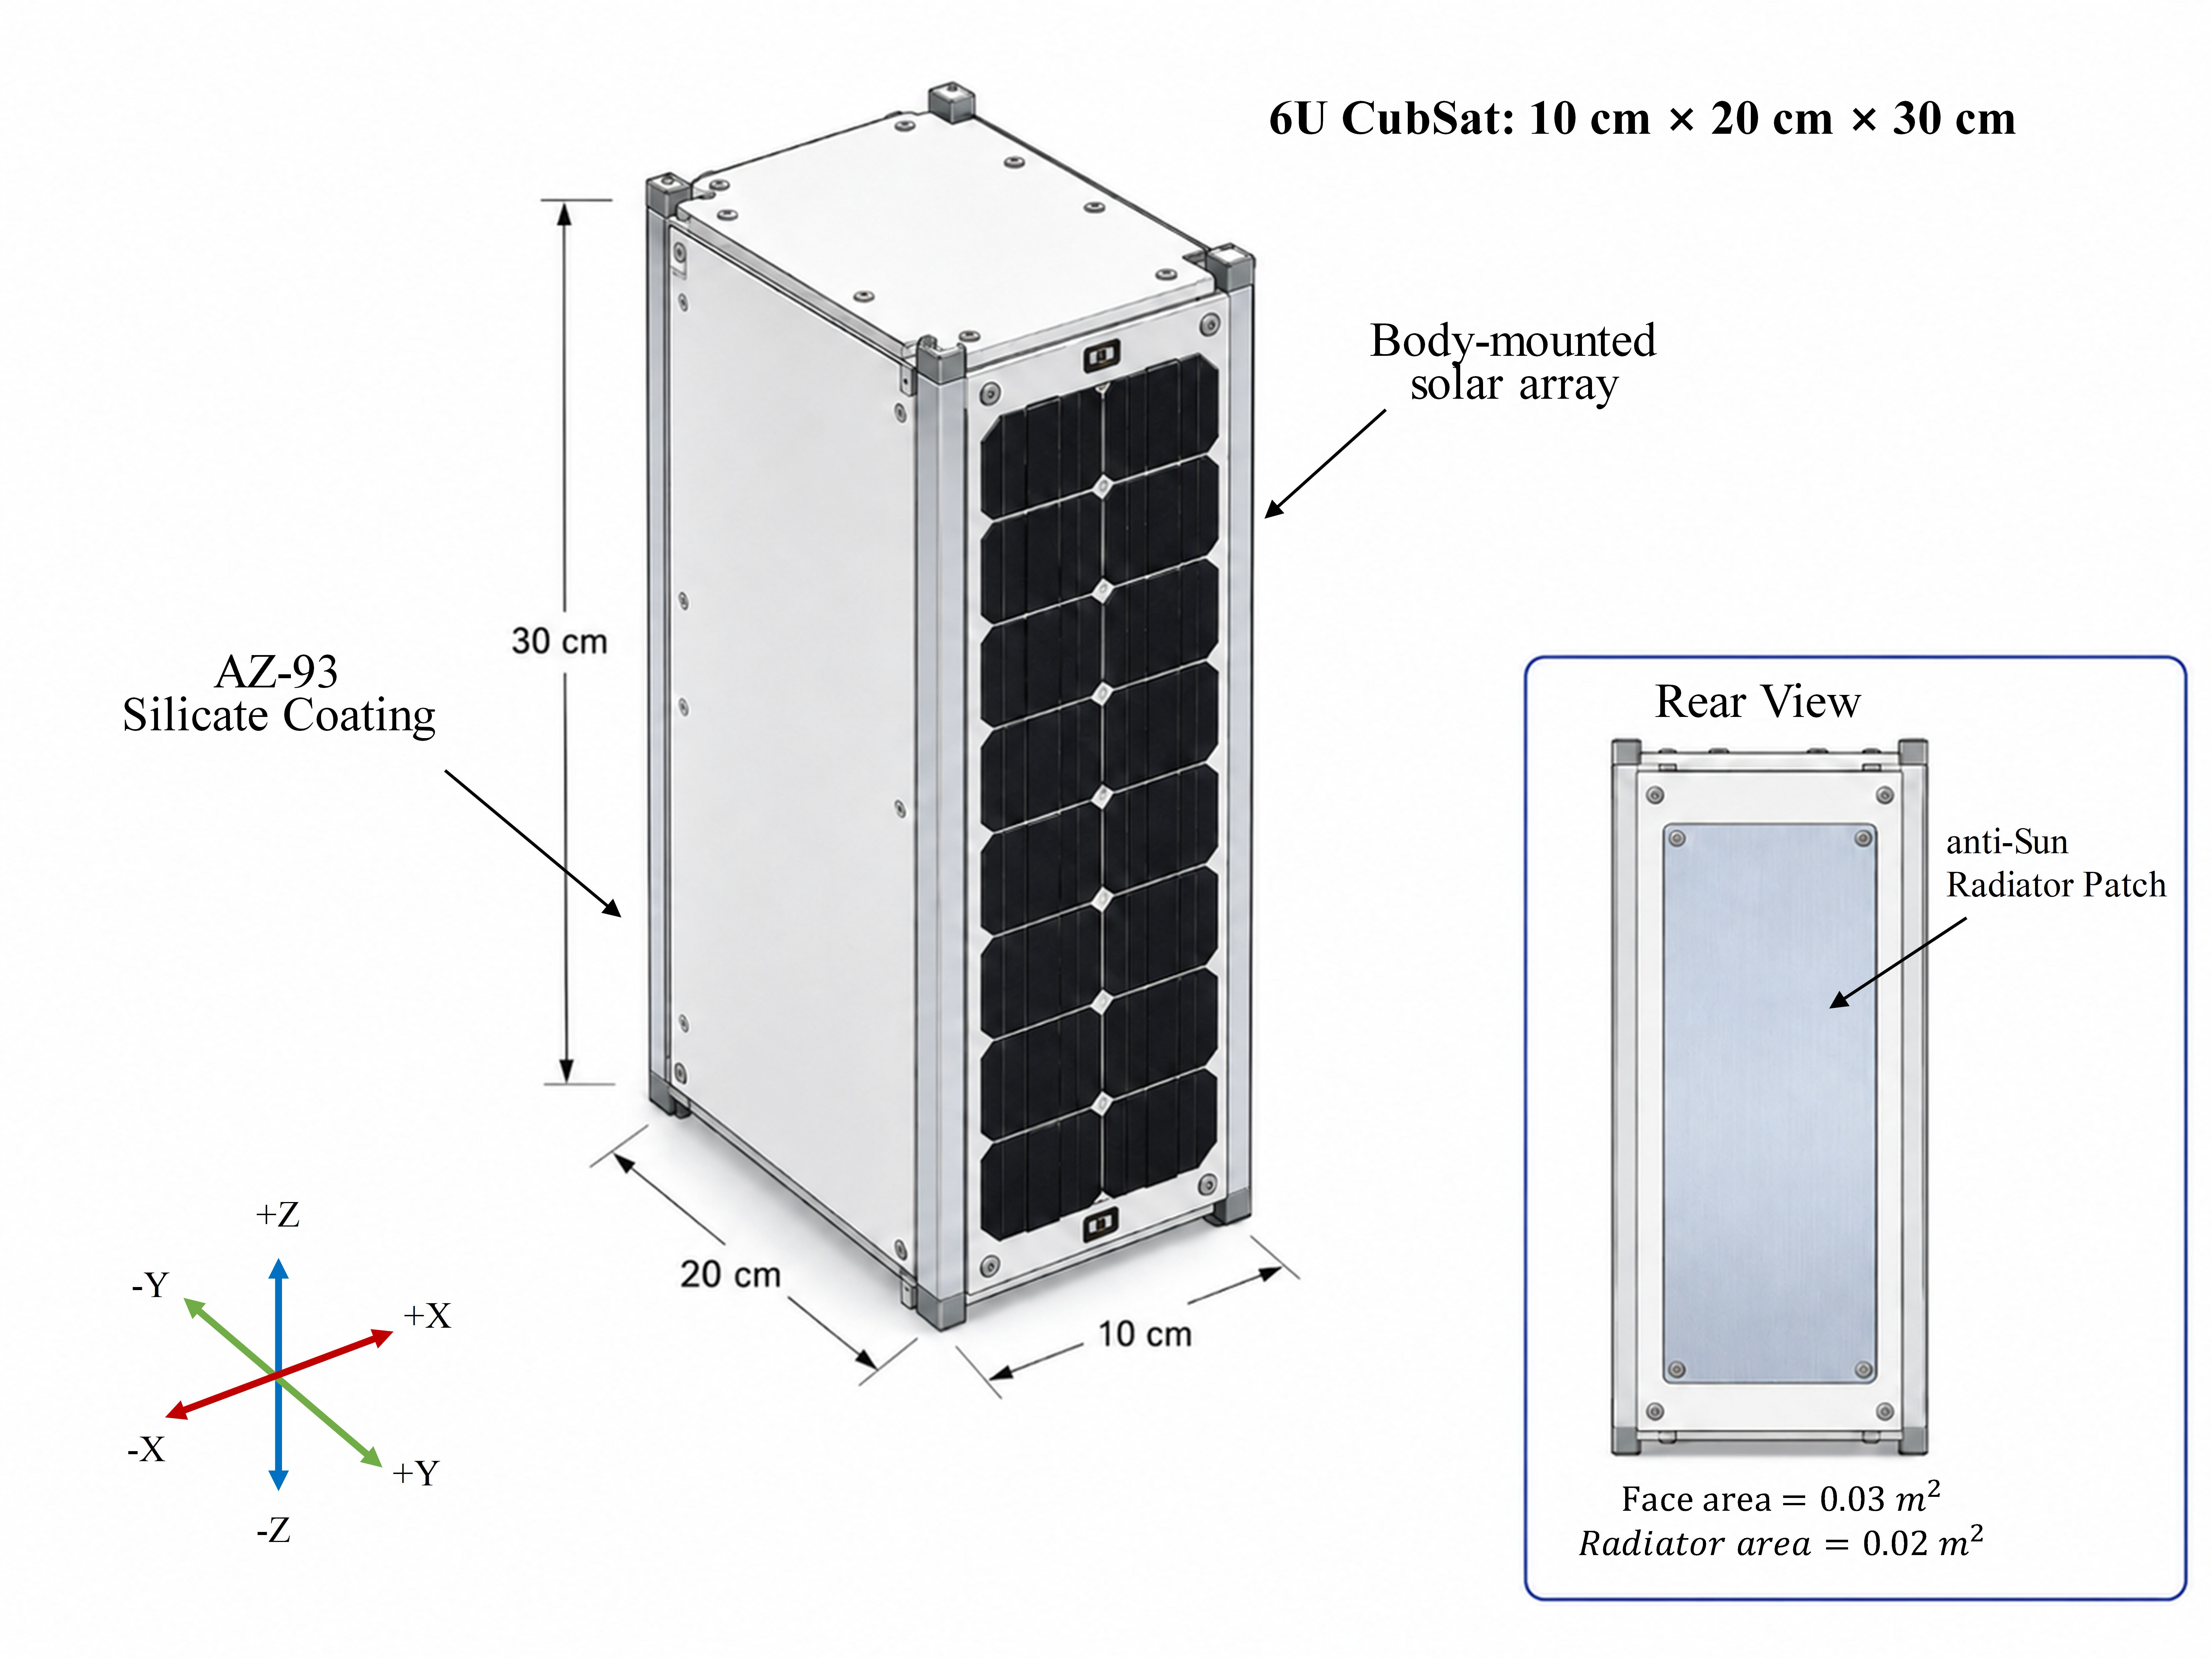
\includegraphics[width=0.65\textwidth]{thermal_zoning.png}
\caption{卫星被动热分区设计布局（Redesign v2），展示了 $+Y$ 迎阳面的太阳电池阵列、外壳表面的 AZ-93 白漆以及 $-Y$ 背阳面的银 FEP 散热板。}
\end{figure}

\section{工况仿真分析结果}
采用 Redesign v2 被动热设计后，所有仿真工况成功收敛至合格限值内。表 3 给出了详细数据。

\begin{table}[H]
\centering
\caption{重设计后各工况下结点稳态温度范围}
\vspace{0.2cm}
\resizebox{\textwidth}{!}{%
\begin{tabular}{lccc}
\toprule
\textbf{结点 ID} & \textbf{标称工况 ($\beta = 65^\circ$) [$^\circ$C]} & \textbf{极端热工况 ($\beta = 74^\circ$) [$^\circ$C]} & \textbf{极端冷工况 ($\beta = 60^\circ$) [$^\circ$C]} \\
\midrule
电池包 & 14.8 至 15.1 & 35.0 至 35.4 & 5.0 至 10.0 \\
航电单机 & 16.4 至 17.1 & 38.1 至 39.2 & -0.8 至 0.8 \\
载荷相机 & 14.1 至 17.7 & 34.0 至 40.3 & -1.7 至 -0.5 \\
结构框架 & 13.2 至 14.2 & 33.5 至 34.8 & -2.2 至 -0.1 \\
加热器占空比 & 0.0\% & 0.0\% & 36.7\% \\
加热器能耗 & 0.0 Wh & 0.0 Wh & 5.92 Wh/轨道 \\
\bottomrule
\end{tabular}%
}
\end{table}

\section{散热板面积与加热能耗权衡研究}
对散热板面积 $A_{\text{rad}}$ 进行 $0.02$ 至 $0.06\text{ m}^2$ 的参数扫频，对比高温峰值与低温加热器能耗（表 4）。

\begin{table}[H]
\centering
\caption{散热板面积尺寸权衡结果}
\vspace{0.2cm}
\resizebox{\textwidth}{!}{%
\begin{tabular}{ccccc}
\toprule
\textbf{面积 [$m^2$]} & \textbf{热工况航电峰值 [$^\circ$C]} & \textbf{冷工况电池最低值 [$^\circ$C]} & \textbf{冷工况加热占空比 [\%]} & \textbf{冷工况加热能耗 [Wh]} \\
\midrule
0.02 & 39.17 & 5.00 & 36.7\% & 5.92 \\
0.03 & 34.87 & 5.00 & 41.5\% & 6.69 \\
0.04 & 31.15 & 5.00 & 49.0\% & 7.90 \\
0.05 & 27.80 & 5.00 & 63.6\% & 10.26 \\
0.06 & 24.81 & 4.99 & 60.9\% & 9.81 \\
\bottomrule
\end{tabular}%
}
\end{table}

\section{可视化图表与设计分析}
结点的瞬态温度响应及参数扫频权衡曲线见下图。图 4 展示了在全日照极端热工况下各结点的温度历程（已收敛至稳态）。图 5 展示了随着散热板面积变化，热工况下航电峰值温度与冷工况下电池最低温度的双轴权衡变化趋势。

\begin{figure}[H]
\centering
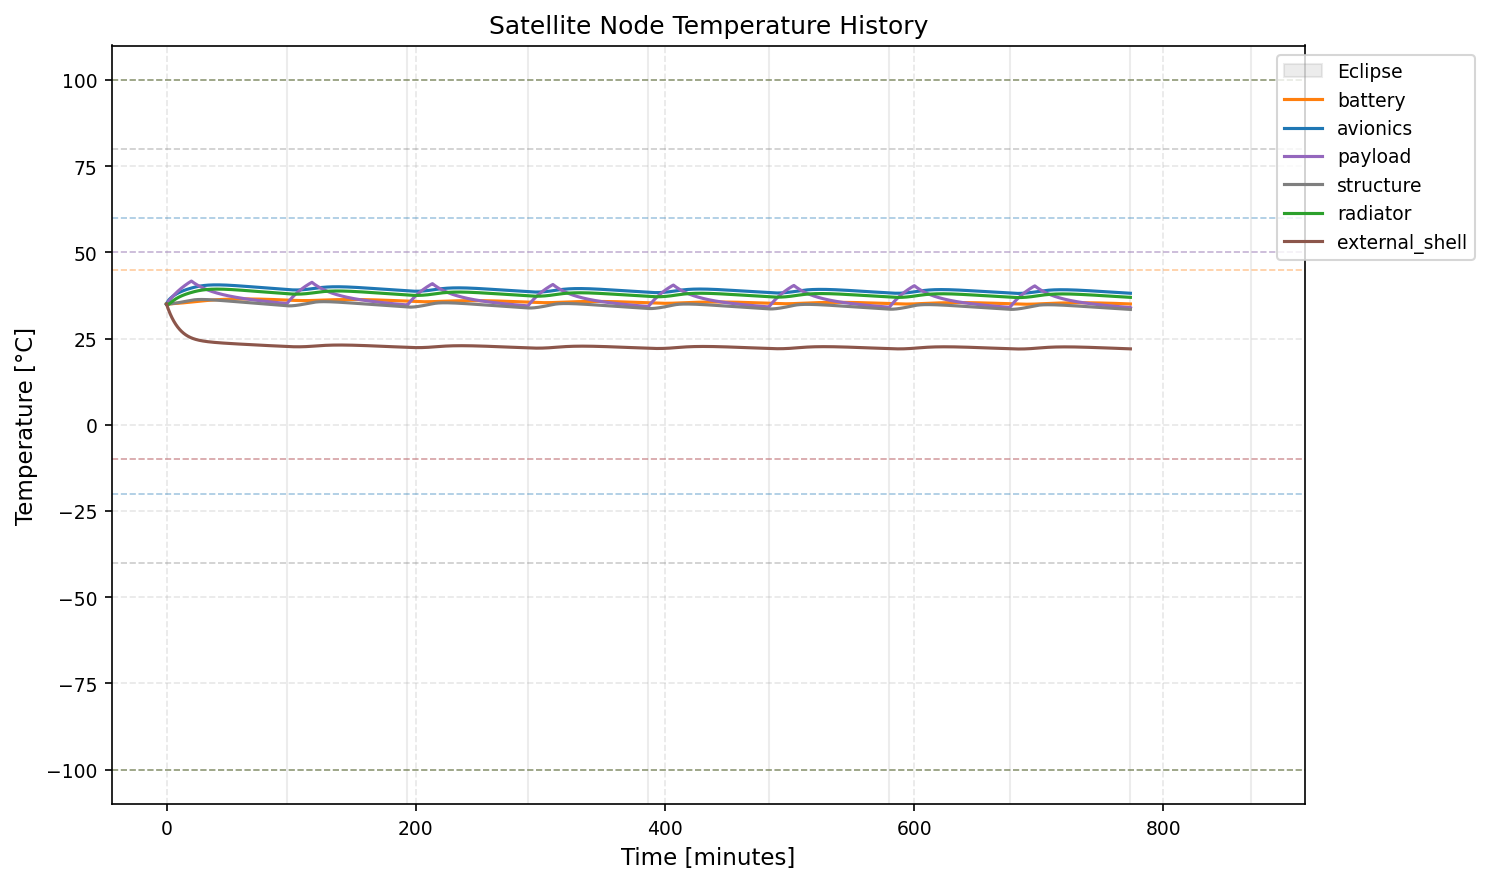
\includegraphics[width=0.7\textwidth]{../outputs/bounding_hot/temperature_history.png}
\caption{极端热工况下各结点温度历程（$\beta = 74^\circ$，晨昏 SSO 至日全日照）}
\end{figure}

\begin{figure}[H]
\centering
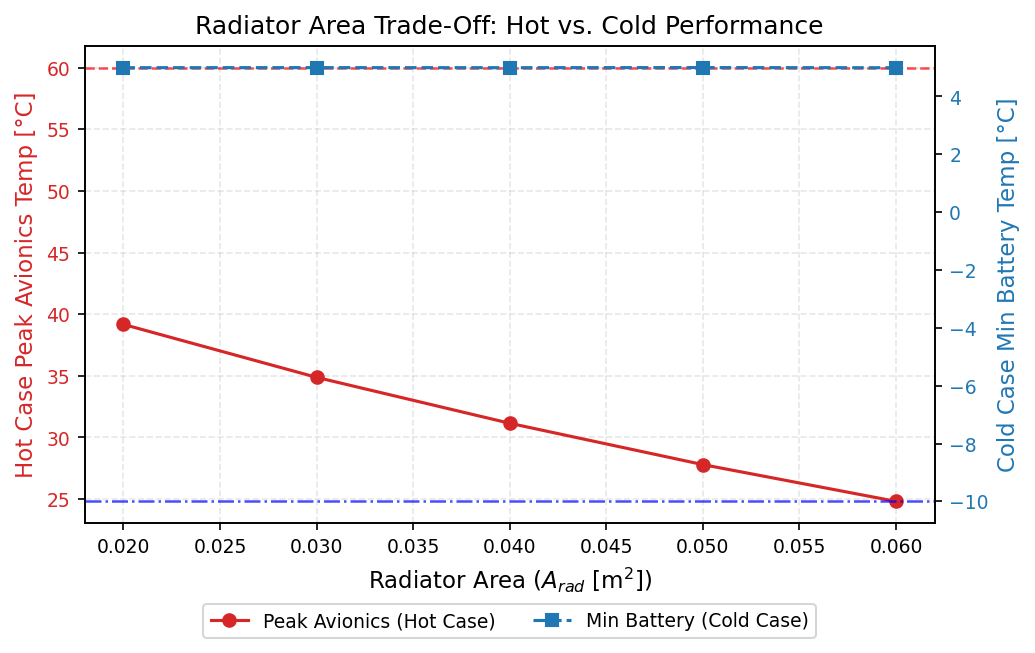
\includegraphics[width=0.7\textwidth]{../outputs/trades/radiator_area_system_trade.png}
\caption{散热器尺寸双轴权衡曲线（极端热工况航电峰值温度 vs. 极端冷工况电池最低温度）}
\end{figure}

\section{结论}
本报告表明，通过合理的物性表面分区、朝阳面光电转换偏置修正和完美的背阴散热板布局，可以在 600 km 全日照晨昏轨道下优雅地解决 6U 立方星的超温失效。散热器尺寸权衡设计对节省整星功耗预算具有至关重要的作用。

\end{document}
